\begin{figure}
    \centering
    \begin{circuitikz}[american, voltage shift=0.5]
    \ctikzset{bipoles/oscope/waveform=square}
    \draw
    (0,0)to [R,l=$R$,i=$i_R$,v=$V_R$] (4,0)
    to [C,l=$C$,v=$V_C$](4,-3)
    to [short,-](0,-3)
    (4,0) to [short,-](6,0)
    to [rmeterwa,t=V](6,-3)
    to [short,-](4,-3)
    (0,0) to [oscope,v_=$V_g$](0,-3);
\end{circuitikz}
    \caption{Circuito}
    \label{fig: Circuito}
\end{figure}
\section{Esperienza 2}
In questa esperienza di laboratorio si è cercato di comprendere al meglio il comportamento di elementi passivi come condensatori e resistenze interfacciandosi con strumenti di laboratorio come generatori di funzione ed oscilloscopi.
In particolare il circuito che maggiormente si è preso in esame è quello rappresentato nella figura \ref{fig: Circuito}.Si è inoltre cercato di capire l'errore che gli esperimenti di laboratorio portano a commettere se utilizzati inconsapevolmente.
\subsection{2.1}
Come prima esperienza si è cercato di stimare la costante di tempo $\tau$. Quest'ultima è definita a partire dalla risposta della differenza di potenziale ai capi della capacità. Questa costante può essere stimata sia durante la carica che la scarica del condensatore. Per simulare in laboratorio questo aspetto si è impostato il potenziale ai capi del genearatore come un onda quadra.
\subsection{Scarica del consensatore $R=15k\Omega $ $C=1nF$}
La $\tau$ teorica in questo caso può essere calcolata tramite la formula $\tau=RC$, pertanto in questo caso $\tau=15\mu s$. Dalla teoria dell'elettromagnetismo la forma teorica che dovrebbe avere il potenziale ai capi di $C$ vale:
\begin{equation}
\label{eq 1}
    V_C(t)=V_{C0}e^{-t/\tau}
\end{equation}
Ove $V_{C0}$ è la tensione iniziale ai capi $C$ che nel caso in questione è pari a $3V$.\\
Si è quindi fatto un fit dei dati sperimentali con la funzione \ref{eq 1} modificato con un parametro $t_0$ per accomodare al meglio il fit. Si è quindi usato il seguente modello:
\begin{equation}
    V_C(t)=V_{C0}e^{-(t-t_0)/\tau}
\end{equation}
Il risulato ottenuto è quello riportato in figura \ref{fig:Scarica RC1}
\begin{figure}
    \centering
    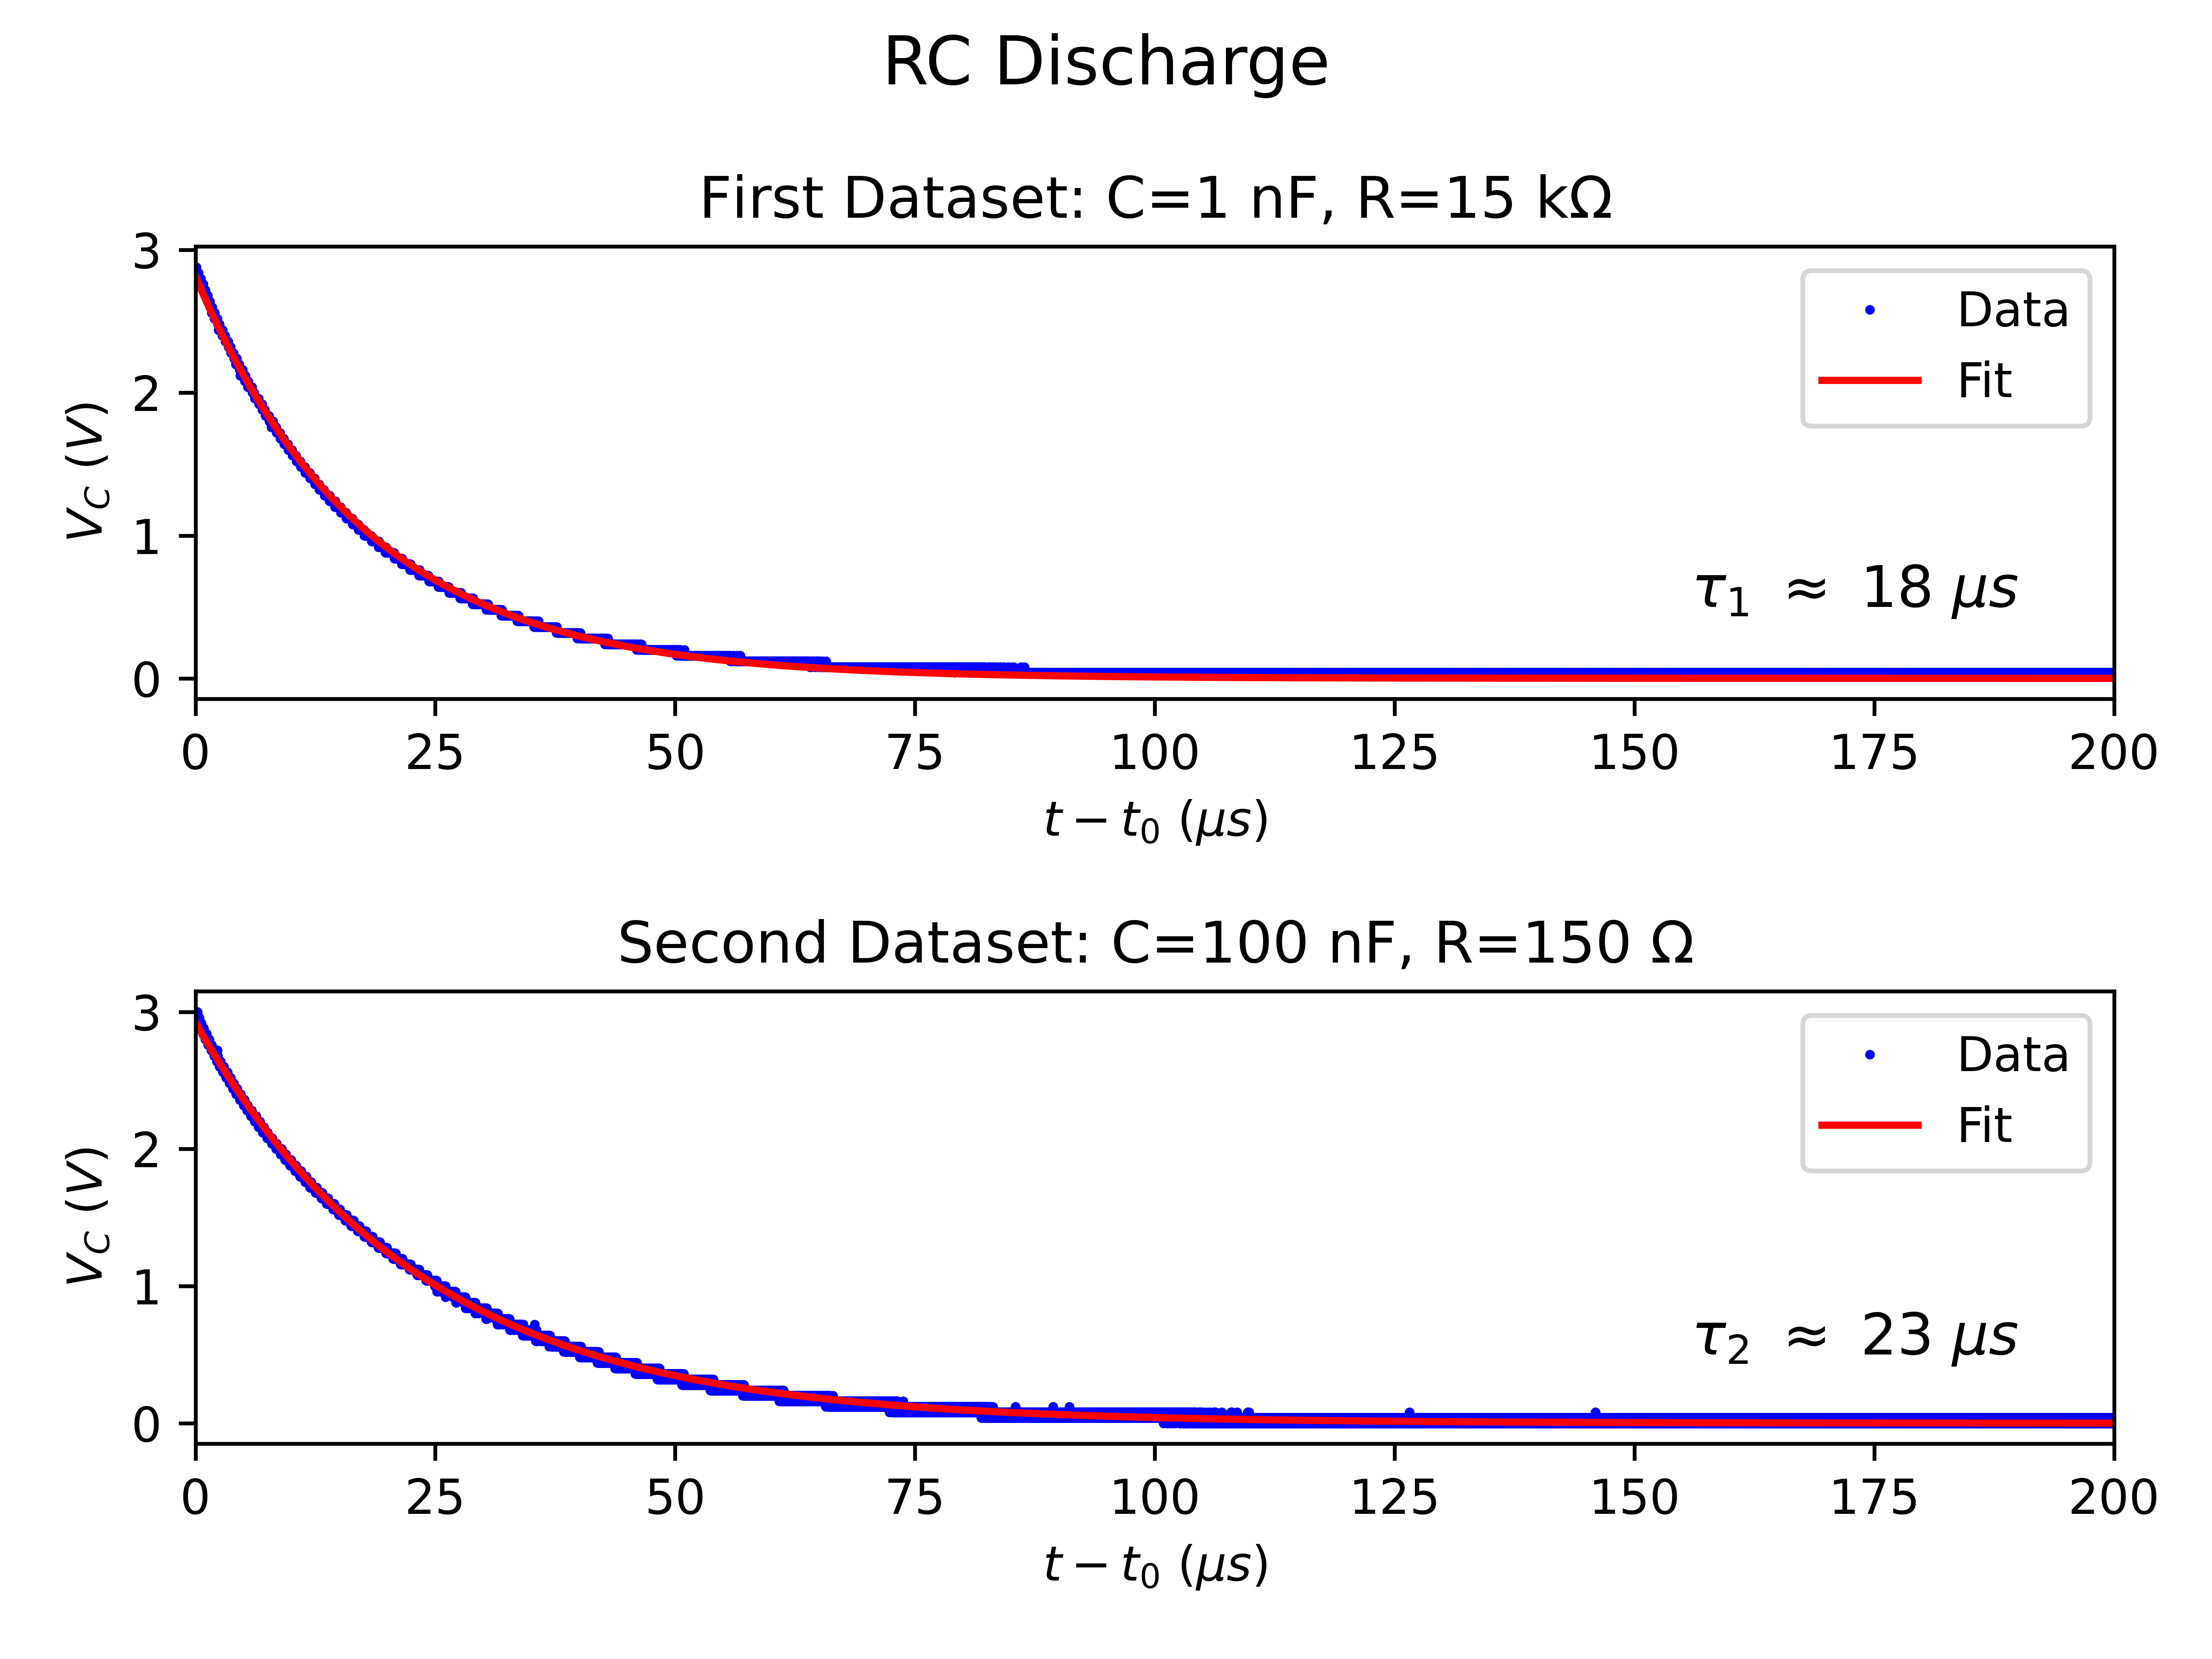
\includegraphics[trim=0 160 0 30, clip, width=\textwidth]{scarica_RC.png}
    \caption{Scarica RC}
    \label{fig:Scarica RC1}
\end{figure}
\subsection{Propagazione dell'errore}
Dalla teoria della propagazione dell'errore e dall'equazione $\tau=RC$ si ha:
\begin{equation}
    \frac{\Delta\tau}{\tau}=\frac{\Delta R}{R}+\frac{\Delta C}{C}
\end{equation}
Si è stimato l'errore su $C$ come pari al $20\%$ mentre la resistenza $R$ misurata con il multimetro è $14.96$\unit{\kohm} . Tramite il datasheet del multimetro si è stimato un $\Delta R = 0.15 $\unit{\kohm}. Pertanto:
\begin{equation}
    \Delta \tau = 3\unit{\us}
\end{equation}
Pertanto 
\begin{equation*}
    \tau=(15\pm 3) \unit{\us}
\end{equation*}
Eseguendo un fit dei dati tramite la relazione \ref{eq 1} si è ottenuta $\tau=18\unit{\us}$ che è all'interno del range della barra di errore.
\subsection{2.1.3}
Uno schema circuitale di questo tipo può essere adottato per eseguire semplici operazioni matematiche come l'integrazione e la derivazione.
\subsection{Scarica del consensatore $R=150$ \unit{\ohm} $C=100$\unit{\nF}}
Si è poi ripetuta la medesima esperienza, utilizzando però diversi valori per capacità e resistenza. Si è scelto il valore di $150 $\unit{\ohm} per la resistenza poichè, così facendo, essa diventa comparabile con la resistenza interna dell'oscilloscopio, del valore nominale di $50$\unit{\ohm}. \\
Nella prima parte dell'esperienza si è volutamente omessa questa considerazione poichè il rapporto $\frac{R_{g}}{R}$ è insignificante a tutti gli scopi pratici. 
La trattazione fisica del circuito è chiaramente la stessa del caso precedente, basta infatti considerare un circuito $RC$ equivalente con $R_{eq}$ pari a $ R + R_{g}=200\unit{\ohm}$ come nello schema circuitale \ref{scarica R 150}.\\
Nel calcolo della $\tau$ sarà pertanto necessario considerare la $R_{eq}$ ottenendo quindi:
\begin{equation*}
    \tau=(20\pm 3)\unit{\us}
\end{equation*}
Eseguendo il fit dei dati la $\tau$ misurata sperimentalmente è pari a $\tau=23\unit{\us}$
\begin{figure}
    \centering
    \begin{circuitikz}[american, voltage shift=0.5]
    \ctikzset{bipoles/oscope/waveform=square}
    \draw
    (0,0)to [R,l=$R_{g}$] (2,0) to[R,l=$R$] (5,0)
    to [C,l=$C$,v=$V_C$](5,-3)
    to [short,-](0,-3)
    (5,0) to [short,-](7,0)
    to [rmeterwa,t=V](7,-3)
    to [short,-](5,-3)
    (0,0) to [oscope,v_=$V_g$](0,-3);
    \draw[draw=black] (0.25,-0.8) rectangle ++(4.25,2);
    \node at (2.3,1.5){$R_{eq}$};
    \end{circuitikz}
    \label{scarica R 150}
    \caption{Schema circuitale}
\end{figure}
\begin{figure}
    \centering
    \includegraphics[trim=0 0 0 177, clip, width=\textwidth]{Scarica_RC.png}
    \caption{Caption}
    \label{fig:enter-label}
\end{figure}
Durante l'analisi si è notato che la tensione erogata dal generatore è deformata. Quest'osservazione si spiega ricordando che la misura della tensione viene effettuata a valle della resistenza del generatore che risulterà pari a 
\begin{equation}
    V_{mis}(t)=V_g-R_g I=V_g-R_g\frac{V_g-V_C(t)}{R_g+R}=\frac{R}{R_g+R}V_g+\frac{R_g}{R_g+R}V_C(t)
\end{equation}
Compare quindi un contributo dovuto alla tensione ai capi del condensatore che modifica la te nsione misurata sull'oscilloscopio. Chiaramente per $R>>R_g$ si ha $V_{mis}(t)\xrightarrow{}V_g$ che riconduce quindi al caso precedente. 
\subsubsection{Carica del condensatore}
Grazie all'ausilio del generatore d'onda quadra è stato possibile con una sola misura ricavare il grafico della carica del condensatore nei vari casi i cui grafici si possono trovare in figura \ref{fig:Carica condensatore}.
\begin{figure}
    \centering
    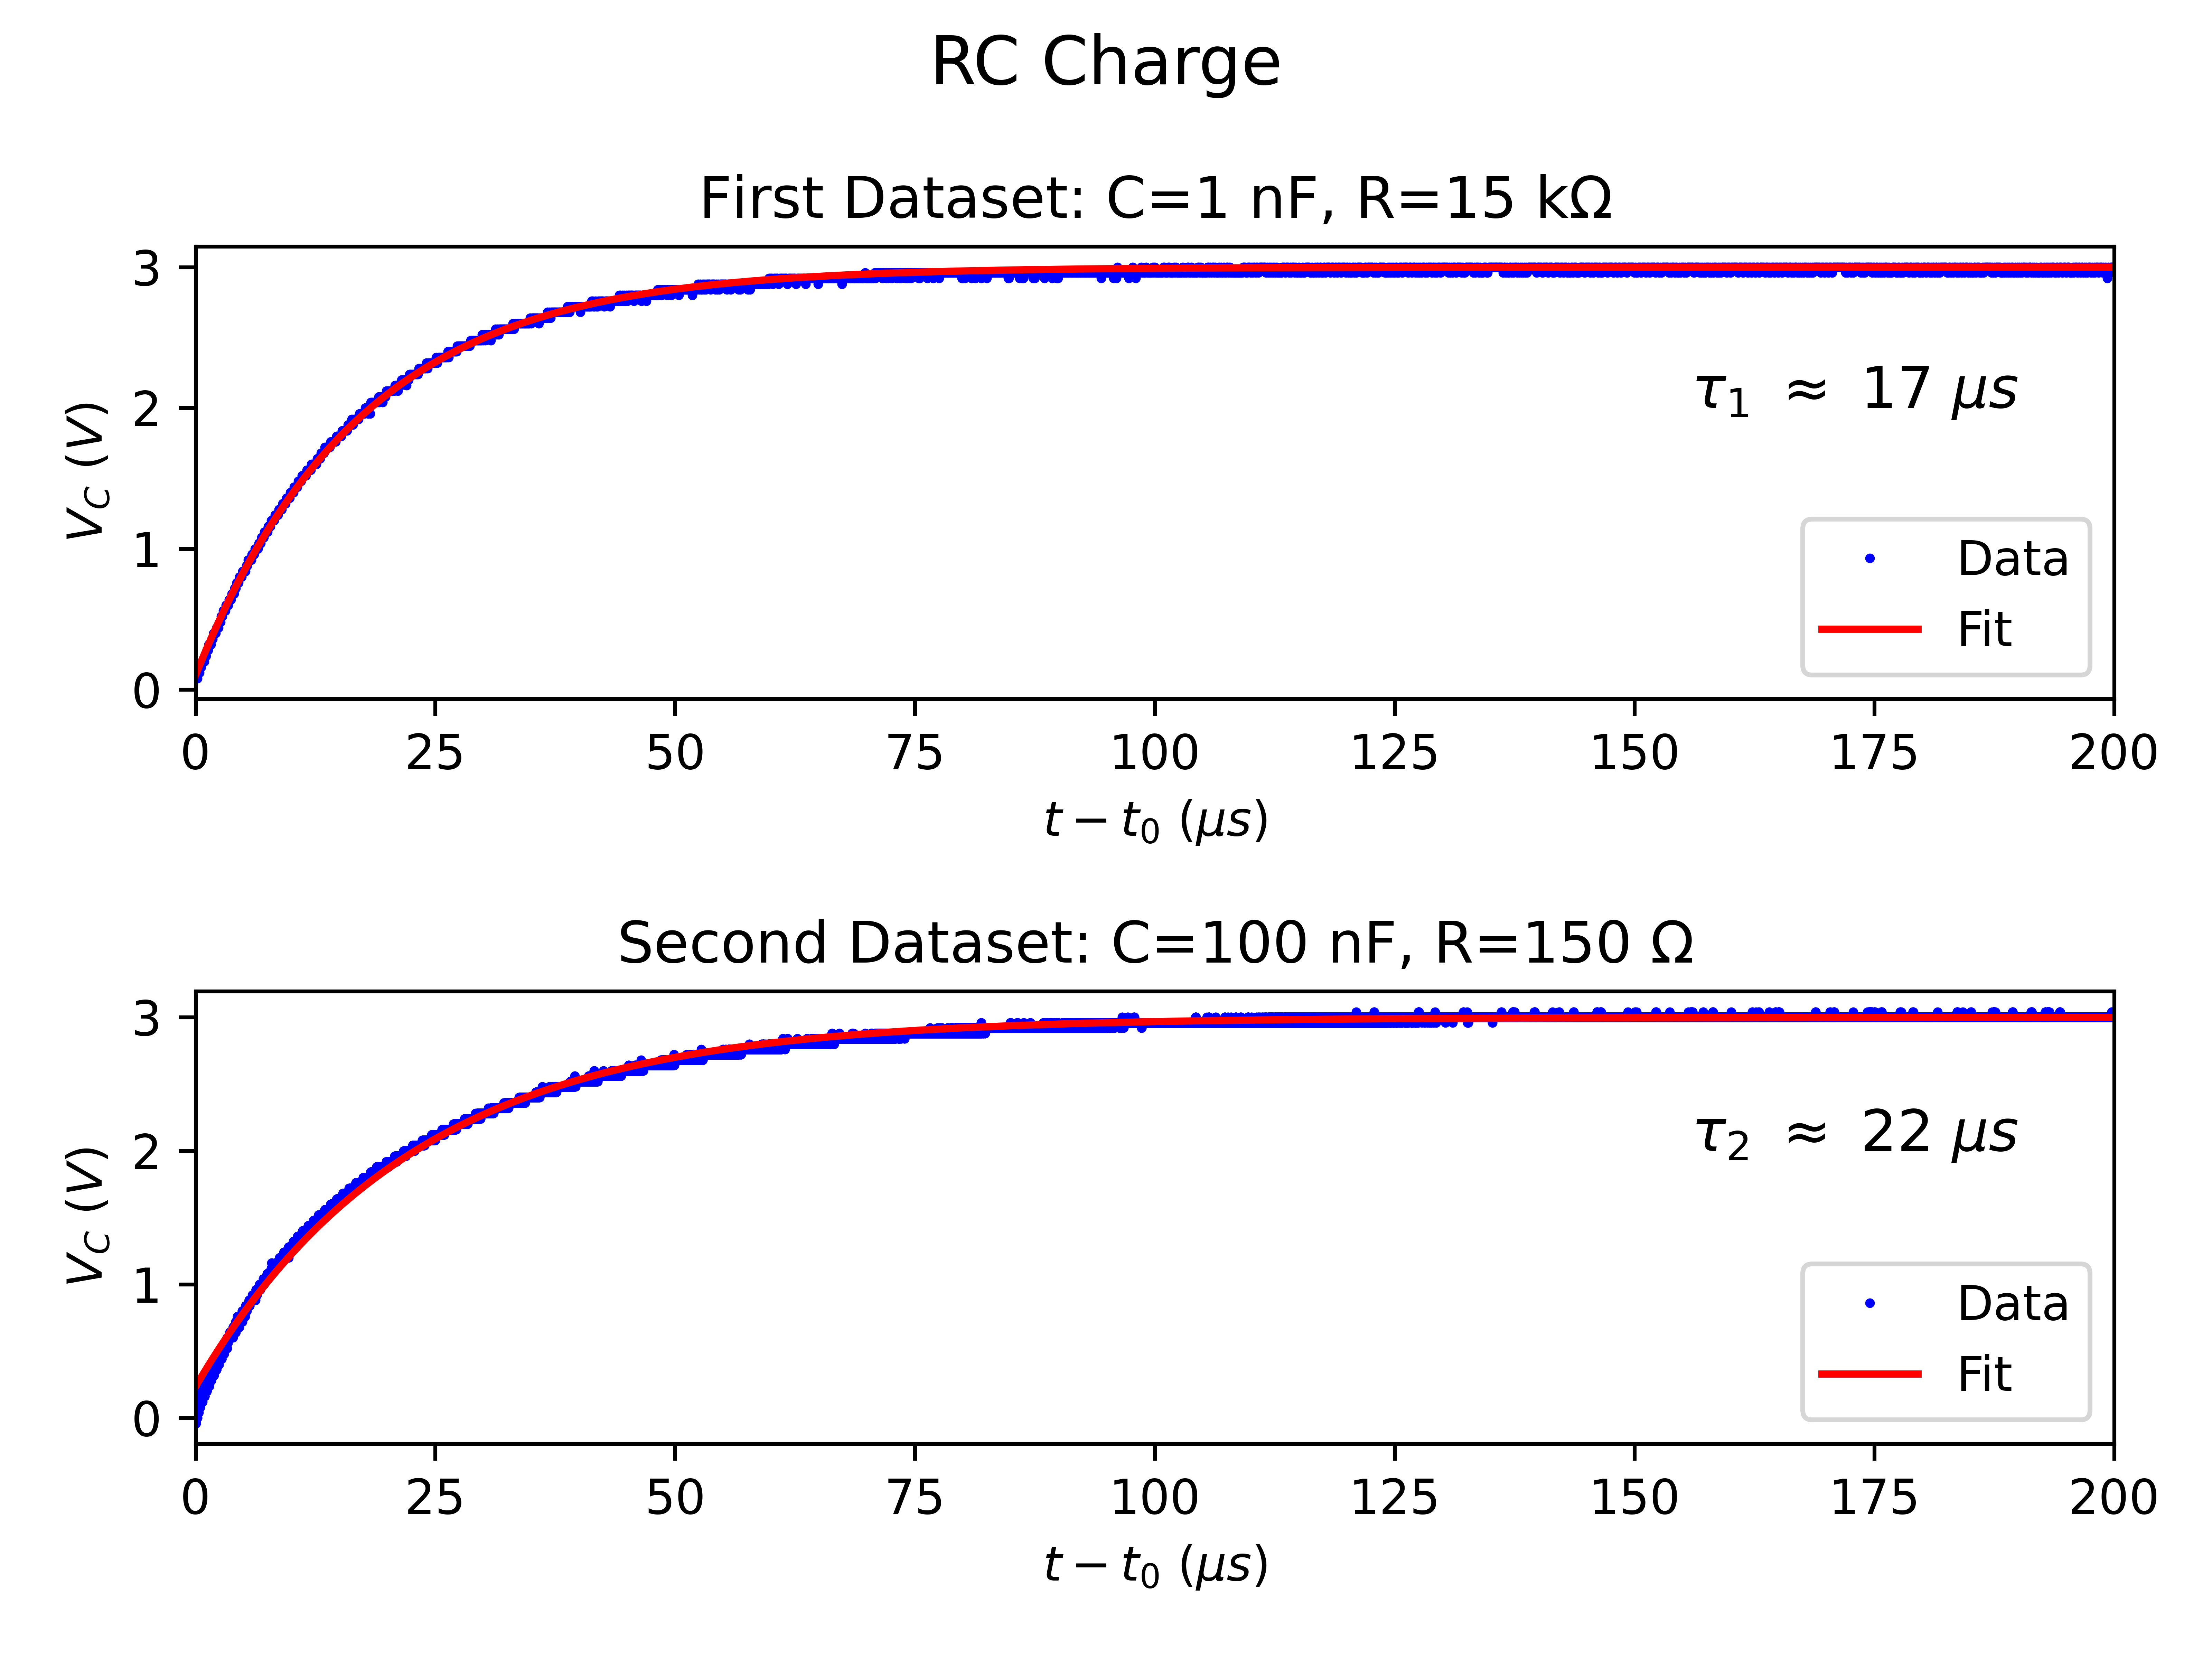
\includegraphics[scale=0.7]{Carica_RC.png}
    \caption{Carica condensatore}
    \label{fig:Carica condensatore}
\end{figure}
\begin{figure}
    \centering
    \begin{circuitikz}[american, voltage shift=0.5]
    \ctikzset{bipoles/oscope/waveform=square}
    \draw
    (0,0)to [R,l=$R_1$] (3,0)
    to [R,l=$R_2$,](3,-3) -- (0,-3);
    \draw (3,0) to [R,l=$R$](6,0)
    to [C,l=$C$](9,0)
    to[L,l=$L$,v=$v_L$](9,-3) -- (0,-3) to [oscope,v^<=$V_g$](0,0);
    \draw (9,0) -- (11,0) to [rmeterwa,t=V](11,-3) --(9,-3);
\end{circuitikz}
    \caption{Circuito}
    \label{fig: Circuito}
\end{figure}